\documentclass[12p]{article}

\title{\huge Przegląd metod całkowania numerycznego}
\date{Analiza Numeryczna (M) - P2 - Zadanie P1.9\\ 28 listopada 2020}
\author{\Large Kacper Kingsford}

\usepackage[T1]{fontenc}
\usepackage[utf8]{inputenc}
\usepackage{lmodern}
\usepackage[margin=0.9in]{geometry}
\usepackage{amsthm}
\usepackage{amsmath}
\usepackage{tikz}
\usepackage{amsfonts} 
\usepackage{changepage}

\makeatletter
\let\sv@endpart\@endpart
\def\@endpart{\thispagestyle{empty}\sv@endpart}
\makeatother


\usepackage{graphicx}
\graphicspath{ {/Desktop/programowanie/ANM/P2/doc/} }
\renewcommand*\contentsname{Spis treści}
\usepackage{listings}
\usepackage{xcolor}

\definecolor{codegreen}{rgb}{0,0.6,0}
\definecolor{codegray}{rgb}{0.5,0.5,0.5}
\definecolor{codepurple}{rgb}{0.58,0,0.82}
\definecolor{backcolour}{rgb}{0.95,0.95,0.92}
\usepackage{ragged2e}

\lstdefinelanguage{Julia}%
{
    morekeywords={%
        exit,whos,edit,load,is,isa,isequal,typeof,tuple,ntuple,uid,hash,finalizer,convert,promote,%
        subtype,typemin,typemax,realmin,realmax,sizeof,eps,promote_type,method_exists,applicable,%
        invoke,dlopen,dlsym,system,error,throw,assert,new,Inf,Nan,pi,im,begin,while,for,in,return,%
        break,continue,macro,quote,let,if,elseif,else,try,catch,end,bitstype,ccall,do,using,module,%
        import,export,importall,baremodule,immutable,local,global,const,Bool,Int,Int8,Int16,Int32,%
        Int64,Uint,Uint8,Uint16,Uint32,Uint64,Float32,Float64,Complex64,Complex128,Any,Nothing,None,%
        function,type,typealias,abstract%
  },%
  sensitive=true,%
  morecomment=[l]\#,%
  morecomment=[n]{\#=}{=\#},%
  morestring=[s]{"}{"},%
  morestring=[m]{'}{'},%
}[keywords, comments, strings]%

\lstset{%
    language         = Julia,
    basicstyle       = \ttfamily,
    keywordstyle     = \bfseries\color{blue},
    columns          = fullflexible,
    stringstyle      = \color{magenta},
    commentstyle     = \color{gray},
    showstringspaces = false,
    numbers          = left,
    xleftmargin      = 2em
}


\begin{document}
\begin{titlepage}

\maketitle
\thispagestyle{empty}
\begin{center}
	\textbf{\large Streszczenie}
\end{center}
\par Całkowanie numeryczne to metoda numeryczna polegająca na przybliżonym obliczaniu całek oznaczonych. Proste metody polegają na przybliżeniu całki za pomocą odpowiedniej sumy ważonej wartości całkowanej funkcji w kilku punktach. Aby uzyskać dokładniejsze przybliżenie dzieli się przedział całkowania na niewielkie fragmenty. Ostateczny wynik jest sumą oszacowań całek w poszczególnych podprzedziałach. Najczęściej przedział dzieli się na równe podprzedziały, ale bardziej wyszukane algorytmy potrafią dostosowywać krok do szybkości zmienności funkcji. 
\par Ze względu na częstotliwość występowania całek oznaczonych w matematyce, istotne jest to, żeby móc je dokładnie aproksymować. Niniejsze sprawozdanie jest podsumowaniem eksperymentu numerycznego polegającego na obliczaniu całek  metodą trapezów oraz Romberga.


\end{titlepage}

\newpage

\tableofcontents

\newpage

\section{Metody całkowania numerycznego}
Całki oznaczone mogą być nieskończone. Spójrzmy choćby na funkcje
\[ t(x) = e^{-x^2}\]
\begin{center}
\includegraphics[scale=0.3]{img3.png}
\end{center}
Aby wyeliminować ten problem będziemy przybliżać funkcje które całkujemy innymi, których całki da się łatwo policzyć: 
\[ \int_{a}^{b} f(x) \,dx  \approx \int_{a}^{b} g(x) \,dx \]
Będziemy stosować interpolacje wielomianową. Weźmy:
\[ g(x) = \sum_{i=1}^{n} f(x_{i})\prod_{j=0, j \neq i
}^{n} \frac{x-x_{j}}{x-x_{i}}  \]
wtedy
\[ \int_{a}^{b} f(x) \,dx  \approx \int_{a}^{b} g(x) \,dx = \sum_{i=1}^{n} f(x_{i})\prod_{j=0, j \neq i
}^{n} \int_{a}^{b}  \frac{x-x_{j}}{x-x_{i}}dx .\]
Niech
\[ A_{i} = \int_{a}^{b}  \frac{x-x_{j}}{x-x_{i}}dx\]
zatem
\[ \int_{a}^{b} f(x) \,dx  \approx \sum_{i=1}^{n} A_{i}f(x_{i}).\]
Wzór ten nazywamy kwadraturą.


\subsection{Metoda złożonych trapezów}

Spójrzmy na wzór trapezów. Weźmy $n=1 \implies x_{0} = a, \;\; x_{1} = b$. Wtedy \[A_{0} = \int_{a}^{b} \frac{b-x}{b-a}dx = \frac{1}{2}(b-a), A_{1} = \int_{a}^{b} \frac{x-a}{b-a}dx = \frac{1}{2}(b-a)\]
\[ \int_{a}^{b} f(x) \,dx \approx \frac{1}{2}(b-a)[f(a)+f(b)].\]
Łatwo sprawdzić, że wzór ten jest dokładny, tylko dla $f \in \pi_{1}$.
\begin{center}
\includegraphics[scale=0.6]{img1.png}
\end{center}

Uogólnijmy tą metode. Podzielmy przedział $[a,b]$ punktami
\[ a = x_{0} < x_{1}<...<x_{n-1} < x_{n} = b\]
na podprzedziały i zastosujmy wzór trapezów:
	\[ \int_{a}^{b} f(x) \,dx = \sum_{i=1}^{n} \int_{x_{i-1}}^{x_i} f(x)dx \approx \frac{1}{2} \sum_{i=1}^{n} (x_{i} - x_{i-1})[f(x_{i-1})+f(x_{i})].\]
Wzór ten jest dokładny gdy wykres funkcji jest łamaną, której wierzchołki mają pierwszą współrzędną $x_{i}$.
W dodatku, jeśli odległości między punktami są równe $x_{i} = a + ih, \;\; h=\frac{b-a}{n}, \;\; h=0,1,...,n$ wzór przyjmuje postać:
\[ \int_{a}^{b} f(x)dx \approx \frac{1}{2}h[f(a)+ 2\sum_{i=1}^{n-1}f(a+ih)+f(b)] \]
\begin{center}
\includegraphics[scale=0.2]{img2.png}
\end{center}

\subsection{Metoda Romberga}

Oznaczmy jako $T(n,1)$ złożony wzór trapezów. Wtedy:
Dla $n=1,2$:
\[ T(1,1) = \frac{b-a}{2} [f(a) + f(b)] \]
\[ T(2,1) = \frac{b-a}{4} [f(a) + 2f(\frac{a+b}{b})+f(b)] \]

Załóżmy, że $f$ ma ciągłe pochodne wszystkich rzędów na $[a,b]$. Wtedy: 
\[ \int_{a}^{b} f(x)dx  = \frac{1}{2}h[f(a)+ 2\sum_{i=1}^{n-1}f(a+ih)+f(b)] + \sum_{i=1}^{\infty}K_{i}h^{2i} \]
gdzie $h = \frac{b-a}{n}$, a stałe $K_{i}$ zależą od pochodnych funkcji $f$. Stąd wynika, że możemy użyć ekstrapolacji Richardsona, aby obliczyć przybliżenie z wyższą dokładnością. Oznaczmy wartość całki przez $I(f)$.
\[ T(1,1) = I(f) + K_{1}h^2 + O(h^4)\]
\[ T(2,1) = I(f) + K_{1}(\frac{h}{2})^2 + O(h^4).\]
Pomijając wyrażenia $O(h^4)$ otrzymamy układ równań, który możemy rozwiązać dla $K_{1}$ oraz $I(f)$. Wartość, którą oznaczamy przez $T(2,2)$ będzie lepszym przybliżeniem:
\[ T(2,2)= T(2,1) + \frac{T(2,1)-T(1,1)}{3}.\]
Stąd wynika, że $I(f) = T(2,2) + O(h^4)$.
Załóżmy, że obliczamy kolejne przybliżenia $T(3,1)$ przy użyciu reguły trapezów z 4 przedziałami. Tak jak poprzednio, możemy użyć ekstrapolacji Richardsona z $T(2,1) $ i $ T(3,1)$, aby uzyskać nowe przybliżenie $T(3,2)$, które jest dokładnie rzędu $O(h^4)$. Teraz mamy dwa przybliżenia $T(2,2) $ oraz $T(3,2)$, które spełniają:
\[ T(2,2) = I(f)+ L_{2}h^4+O(h^6)\]
\[ T(3,2) = I(f)+ L_{2}(\frac{h}{2})^4+O(h^6)\]
dla pewnej stałej $L_{2}$. Wynika stąd, że możemy stosować ponownie ekstrapolacje Richardsona do tych przybliżeń, aby otrzymać nowe przybliżenie z dokładnością do $O(h^6)$. Kontynuując ten proces, możemy otrzymać tak wysoki rząd dokładności jaki chcemy. Uogólniając:
\[ T(n,m) = T(n,m-1) + \frac{T(n,m-1)+T(n-1,m-1)}{4^{n-1}-1}\]


Weźmy wzór trapezów i podstawmy $ n:= 2^n-1:$ i podzielmy przedział $[a,b]$ na równe podprzedziały, otrzymamy:
\[ T(n,1) = \frac{h_n}{2} [f(a) + 2 \sum_{i=1}^{2^{n - 1} -1}f(a+ih_{n})+f(b)], \;\; h_{n} = \frac{b-a}{2^n} .\]
Wyprowadźmy teraz rekurencje na $T(n,1)$ rozbijając sumowanie na dwie sumy zawierające odpowiednio wyrazy nieparzyste 	i parzyste:
\[ T(j,1) = \frac{h_{n}}{2}[f(a)+ \sum_{i=1}^{2^{n-2}}f(a+(2i-1)h_{n})+2 \sum_{i=1}^{2^{n-2}-1}f(a+2ih_{n})+f(b)]\]
\[= \frac{h_{n}}{2}[f(a)+ \sum_{i=1}^{2^{n-2}-1}f(a+2ih_{n})+f(b)]+ \frac{h_{n}}{2} [2\sum_{i=1}^{2^{n-2}}f(a+(2i-1)h_{n})] \]
\[ = \frac{1}{2}T(n-1,1) + h_{n} \sum_{i=1}^{2^{n-2}}f(a+(2i-1)h_{n}.\]
Sumy $T(j,1)$ obliczamy rekurencyjnie tak, aby uniknąć wielokrotnego obliczania wartości funkcji w tych samych punktach.\newpage

Z powyższych obserwacji możemy sformułować algorytm Romberga w pseudokodzie:\\

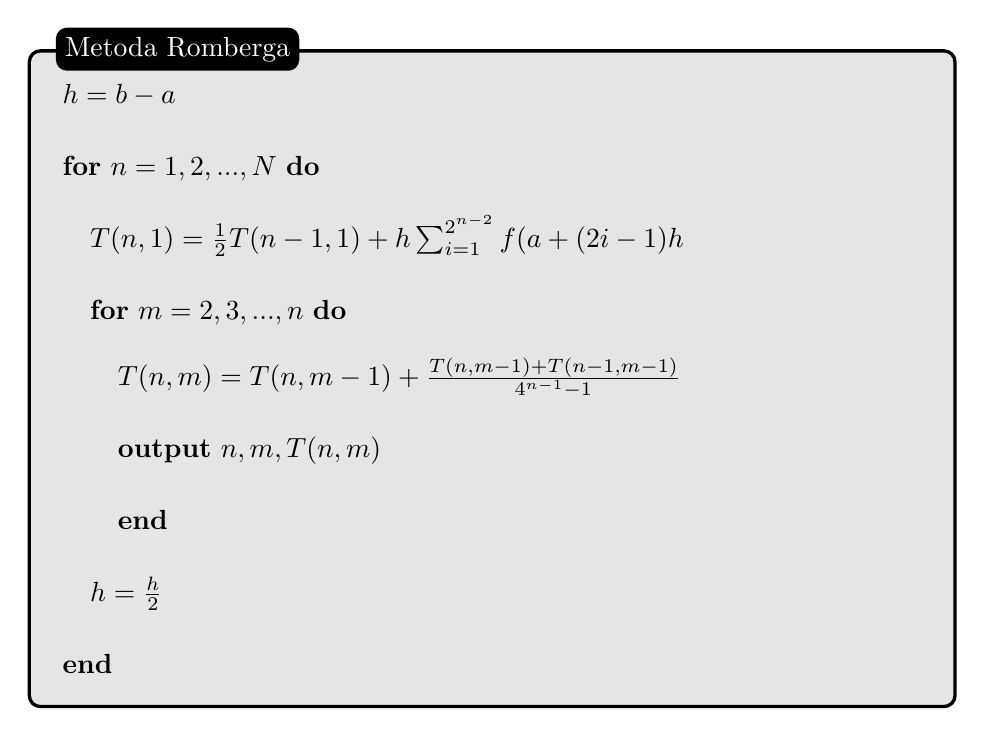
\begin{tikzpicture}
\node [draw={black}, fill=black!10, very thick, rectangle, rounded corners, inner sep=12pt, inner ysep=12pt] (box){%
    \begin{minipage}{.9\textwidth}

$h=b-a$ \\

 \begin{adjustwidth}{0pt}{0pt}
 	\textbf{for} $n=1,2,...,N$ \textbf{do}\\
 \end{adjustwidth}
 
\begin{adjustwidth}{10pt}{0pt}
 $ T(n,1) = \frac{1}{2}T(n-1,1) + h \sum_{i=1}^{2^{n-2}}f(a+(2i-1)h$\\
 
 \end{adjustwidth}
 \begin{adjustwidth}{10pt}{0pt}
 
 \textbf{for} $m=2,3,...,n$ \textbf{do}\\
  \begin{adjustwidth}{10pt}{0pt}
  $T(n,m) = T(n,m-1) + \frac{T(n,m-1)+T(n-1,m-1)}{4^{n-1}-1}$\\
  \end{adjustwidth}
  \begin{adjustwidth}{10pt}{10pt}
\textbf{output} $n,m,T(n,m)$\\
 
 \end{adjustwidth}
   \begin{adjustwidth}{10pt}{0pt}

 \textbf{end}\\
  \end{adjustwidth}

 $h=\frac{h}{2}$\\


 \end{adjustwidth}

\textbf{end}




    \end{minipage}
};
\node[fill={black}, text=white, rounded corners, right=10pt] at (box.north west) {Metoda Romberga};
\end{tikzpicture}

\section{Analiza błędu}


Rozwińmy ze wzoru Taylora funkcję $f$ dla $x = a$ : 
\[ \int_{a}^{b} f(x)dx = \int_{a}^{b} \Big[ f(a)+(x-a)f'(a) + \frac{(x-a)^2}{2!}f''(a) + \frac{(x-a)^3}{3!}f'''(a)+ ... \Big]dx	= hf(a)+\frac{h^2}{2!}f'(a) + \frac{h^3}{3!}f'''(a) + ... \]
Analogicznie dla $x = b$:
\[ \int_{a}^{b} f(x)dx = \int_{a}^{b} \Big[ f(b)+(x-b)f'(a) + \frac{(x-b)^2}{2!}f''(b) + \frac{(x-b)^3}{3!}f'''(b)+ ... \Big]dx	= hf(b)+\frac{h^2}{2!}f'(b) + \frac{h^3}{3!}f'''(b) + ... \]

Dodając obydwie równości stronami i dzieląc przez 2 otrzymujemy:

\[ \int_{a}^{b} f(x)dx = \frac{h}{2}\Big[f(a)+f(b)\Big]+ \frac{h^2}{4}\Big[f'(a) - f'(b)\Big]+ \frac{h^3}{12}\Big[f''(a) + f''(b) \Big]+ ... \]

Powtórzmy całą procedurę z taką różnicą, że będziemy rozwijać funkcje $f'$.

Dla $x=a$:

\[ f'(x) =  f'(a)+(x-a)f''(a) + \frac{(x-a)^2}{2!}f'''(a) + \frac{(x-a)^3}{3!}f^{(4)}(a)+ ...  \;\;\;\;\;\;\;\;\;\;\;\;\;\;(i)\]

oraz $x=b$:

\[ f'(x) =  f'(b)+(x-b)f''(a) + \frac{(x-b)^2}{2!}f'''(b) + \frac{(x-b)^3}{3!}f^{(4)}(b)+ ...  \;\;\;\;\;\;\;\;\;\;\;\;\;\; (ii)\]

Podstawiająca do $(i) \;\; x=b$ mamy:
\[ f'(b) =  f'(a)+ hf''(a) + \frac{h^2}{2!}f'''(a) + \frac{h^3}{3!}f^{(4)}(a)+ ...  \]

Podstawiająca do $(ii) \;\; x=a$ mamy:
\[ f'(a) =  f'(b)- hf''(b) + \frac{h^2}{2!}f'''(b) - \frac{h^3}{3!}f^{(4)}(b)+ ...  \]

Wyznaczając z dwóch poprzednich równości $f''(a) + f''(b)$ otrzymujemy:

\[ f''(a) + f''(b) = \frac{2}{h} \Big[ f'(b) - f'(a) \Big] - \frac{h}{2} \Big[ f'''(a)-f'''(b) \Big]  - \frac{h^2}{6}\Big[ f^{(4)}(a) + f^{(4)}(b)  \Big] + ...\]

Postepując podobnie można wyznaczyć: 

\[ f^{(4)}(a) + f^{(4)}(b) = \frac{2}{h}\Big[ f'''(b) - f'''(a) \Big] + ...\]

Zauważmy, że teraz nasza całka przybiera postać:

\[ \int_{a}^{b}f(x)dx= \frac{h}{2} \Big[f(a) + f(b)  \Big] + \frac{h^2}{12}\Big[ f'(a) -f'(b) \Big] - \frac{h^4}{720}\Big[ f'''(a) - f'''(b) \Big] + ...\]

Podzielmy przedział $[a,b]$ na równe podprzedziały:

\[ \int_{a}^{b} f(x)dx = \sum_{i=0}^{n-1} \int_{x_i}^{x_{i+1}} f(x) dx =  h\Big[ \frac{f(x_{0})}{2} + f(x_{1}) + ... + f(x_{n-1}) + \frac{f(x_{n})}{2} \Big] + \frac{h^2}{12} \Big[  f'(x_{0}) - f'(x_{n})\Big] - \frac{h^4}{720} \Big[  f'''(x_{0}) - f'''(x_{n}) \Big] + ...\]

Otrzymaliśmy złożony wzór trapezów wraz z błędem, który generuje ta metoda.

\section{Opis eksperymentu oraz analiza wyników}

Obliczenia zostały wykonane w języku Julia (wersja 1.5.2.)
przy użyciu 64-bitowej arytmetyki (64 bity przeznaczone na reprezentację mantysy).

Przyjrzyjmy się funkcji $cosx$. Będziemy przybliżać wartość całki:
\[ \int_{0}^{\frac{\pi}{2}} cosx\;dx\]

Wiadomo z elementarnych przekształceń, że:
\[  \int_{0}^{\frac{\pi}{2}} cosx\;dx = sinx |_{0}^{\frac{\pi}{2}} = sin\frac{\pi}{2} - sin0 = 1\]
Spróbujmy obliczyć tą całkę opisanymi wcześniej metodami.
\subsection{Porównanie wyników}

Obliczmy wartość funkcji $compositeTrapezoid(n)$ dla $n = 2,4,...,64$.
Wyniki znajdują się w poniższej tabeli:

\begin{table}[h]
\centering
\begin{tabular}{|c|c|c|}
    \hline
\large $n$   & $compositeTrapezoid(n)$   & $error$
    \normalsize\\
    \hline
    $2^1$      & $7.8539816339744828\cdot10^{-1}$ & $2.15\cdot10^{-1}$\\ \hline
    $2^2$      &   $9.4805944896851990\cdot10^{-1}$ & $5.19\cdot10^{-2}$\\ \hline
    $2^3$      &  $9.8711580097277540\cdot10^{-1}$& $ 1.29\cdot10^{-2}$\\ \hline
    $2^4$      &  $9.9678517188616966\cdot 10^{-1}$ & $3.21\cdot 10^{-3}$\\ \hline
    $2^5$      &  $9.9919668048507226\cdot 10^{-1}$&$8.03\cdot 10^{-4}$ \\ \hline
    $2^6$      &  $9.9979919432001874\cdot 10^{-1}$&$2.01\cdot 10^{-4}$ \\ \hline


\end{tabular}
\center{Tablica 1: Wyniki funkcji $compositeTrapezoid(n)$ dla wybranych wartości $n$.}
\end{table}

Zauważmy, że błąd funkcji bardzo wolno zbiega do zera.\newpage

Zastosujmy więc metodę Romberga. Obliczamy wartości funkcji $ R(n,m) $ dla $n,m = 1,2,...,6$.

Wyniki wartości funkcji znajdujących się na przekątnej tablicy Romberga:

\begin{table}[h]
\centering
\begin{tabular}{|c|c|}
    \hline
\large $n$   & $R(n,n)$   
    \normalsize\\
    \hline
    $1$      & $7.8539816339744828\cdot10^{-1}$ \\ \hline
    $2$      &   $1.0022798774922104$ \\ \hline
    $3$      &  $9.9999156547299273\cdot10^{-1}$\\ \hline
    $4$      &  $1.0000000081440208$ \\ \hline
    $5$      &  $9.9999999999801692\cdot 10^{-1}$\\ \hline
    $6$      &  $1.0000000000000002$ \\ \hline


\end{tabular}
\center{Tablica 2: Wyniki funkcji $R(n,m)$ dla wybranych wartości $n$.}
\end{table}

Tablica przekątniowa błędów metody Romberga:

\begin{center}
\begin{tabular}{|*{6}{c|}}
								\cline{1-1}
  $2.15\cdot 10^{-1}$                        \\ \cline{1-2}
  $5.19\cdot 10^{-2}$ & $2.28\cdot 10^{-3}$                 \\ \cline{1-3}
  $1.29\cdot 10^{-2}$ & $1.35\cdot 10^{-4}$ & $8.43\cdot 10^{-6}$              \\ \cline{1-4}
  $3.21\cdot 10^{-3}$ & $8.30\cdot 10^{-6}$ & $1.24\cdot 10^{-7}$ & $8.14\cdot 10^{-9}$         \\ \cline{1-5}
  $8.03\cdot 10^{-4}$ & $5.17\cdot 10^{-7}$ & $1.90\cdot 10^{-9}$ & $2.98\cdot 10^{-11}$ & $1.98\cdot 10^{-12}$     \\ \hline
  $2.01\cdot 10^{-4}$ & $3.23\cdot 10^{-8}$ & $2.96\cdot 10^{-11}$ & $1.15\cdot 10^{-13}$ & $1.78\cdot 10^{-15}$ & $2.22\cdot 10^{-16}$ \\ \hline
\end{tabular}
\end{center}

Zauważmy, że najlepsze przybliżenie posiada błąd równy $\mathbf{2.22\cdot 10^{-16}}$. Dla metody trapezów wyniósł on $\mathbf{2.01\cdot 10^{-4}}$. Zatem ich iloraz to aż ponad $\mathbf{10^6}$.


\subsection{Funkcja Rungego}

Spójrzmy na kolejny przykład. Będzie to fukcja Rungego:
\[ \int_{-1}^{1} \frac{1}{25x^2 + 1}\]

\begin{center}
\includegraphics[scale=0.3]{img4.png}
\end{center}


Obliczmy wartość funkcji $compositeTrapezoid(n)$ dla $n = 2,4,...,1024$.
Wyniki znajdują się w poniższej tabeli:

\begin{table}[h]
\centering
\begin{tabular}{|c|c|c|}
    \hline
\large $n$   & $compositeTrapezoid(n)$   & $error$
    \normalsize\\
    \hline
    $2^1$      & $7.6923076923076927\cdot10^{-2}$ & $4.72\cdot10^{-1}$\\ \hline
    $2^2$      &   $1.0384615384615385\cdot10^{0}$ & $4.89\cdot10^{-1}$\\ \hline
    $2^3$      &  $6.5716180371352784\cdot10^{-1}$& $ 1.08\cdot10^{-1}$\\ \hline
    $2^4$      &  $5.5689787382316402\cdot 10^{-1}$ & $7.54\cdot 10^{-3}$\\ \hline
    $2^5$      &  $5.4922232360879353\cdot 10^{-1}$&$1.38\cdot 10^{-4}$ \\ \hline
    $2^6$      &  $5.4931218845096019\cdot 10^{-1}$&$4.81\cdot 10^{-5}$ \\ \hline

    $...$      &  $...$&$...$ \\ \hline
    $2^{10}$      &  $5.4936011867707291\cdot 10^{-1}$&$1.88\cdot 10^{-7}$ \\ \hline

\end{tabular}
\center{Tablica 3: Wyniki funkcji $compositeTrapezoid(n)$ dla wybranych wartości $n$.}
\end{table}

Błąd funkcji również bardzo wolno zbiega do 0.\\

Zastosujmy ponownie metodę Romberga. Obliczamy wartości funkcji $ R(n,m) $ dla $n,m = 1,2,...,10$.

Wyniki wartości funkcji znajdujących się na przekątnej tablicy Romberga:

\begin{table}[h]
\centering
\begin{tabular}{|c|c|}
    \hline
\large $n$   & $R(n,n)$   
    \normalsize\\
    \hline
    $1$      & $0.0769231$ \\ \hline
    $2$      &   $1.35897$ \\ \hline
    $3$      &  $0.474801$\\ \hline
    $4$      &  $0.523803$ \\ \hline
    $5$      &  $0.548706$\\ \hline
    $6$      &  $0.549546$ \\ \hline
    $... $      &  $...$ \\ \hline
    $10 $      &  $0.549360$ \\ \hline

    


\end{tabular}
\center{Tablica 4: Wyniki funkcji $R(n,m)$ dla wybranych wartości $n$.}
\end{table}

Tablica przekątniowa błędów metody Romberga:

\begin{center}
\begin{tabular}{|*{10}{c|}}
								\cline{1-1}
  $4.7\cdot 10^{-1}$                        \\ \cline{1-2}
  $4.89\cdot 10^{-1}$ & $8.09\cdot 10^{-1}$                 \\ \cline{1-3}
  $1.07\cdot 10^{-1}$ & $1.92\cdot 10^{-2}$ & $7.45\cdot 10^{-2}$              \\ \cline{1-4}
  $7.53\cdot 10^{-3}$ & $2.58\cdot 10^{-2}$ & $2.63\cdot 10^{-2}$ & $2.55\cdot 10^{-2}$         \\ \cline{1-5}
  $1.37\cdot 10^{-4}$ & $2.69\cdot 10^{-3}$ & $1.15\cdot 10^{-3}$ & $7.51\cdot 10^{-4}$ & $6.53\cdot 10^{-4}$     \\ \cline{1-6}
  $4.81\cdot 10^{-5}$ & $1.81\cdot 10^{-5}$ & $1.60\cdot 10^{-4}$ & $1.81\cdot 10^{-4}$ & $1.84\cdot 10^{-4}$ & $1.85\cdot 10^{-4}$ \\ \cline{1-7}
  $1.20 \cdot 10^{-5}$ & $9.09\cdot 10^{-9}$ & $ 1.20\cdot 10^{-6}$ & $ 1.32\cdot 10^{-6}$& $2.04\cdot 10^{-6}$& $2.22\cdot 10^{-6}$ & $2.27\cdot 10^{-6}$ \\ \cline{1-8}
  $ 3.00\cdot 10^{-6}$ & $5.21\cdot 10^{-10}$ & $5.05\cdot 10^{-11}$ & $1.90\cdot 10^{-8}$& $1.38\cdot 10^{-8}$& $1.19\cdot 10^{-8}$ & $1.13\cdot 10^{-8}$ & $1.12\cdot 10^{-8}$ \\ \cline{1-9}
  $ 7.52\cdot 10^{-7}$ & $3.26\cdot 10^{-11}$ & $1.90\cdot 10^{-14}$ & $8.21\cdot 10^{-13}$& $7.37\cdot 10^{-11}$& $8.73\cdot 10^{-11}$ & $9.03\cdot 10^{-11}$ & $9.10\cdot 10^{-11}$ & $9.11\cdot 10^{-11}$ \\ \hline
  $ 1.88\cdot 10^{-7}$ & $2.03\cdot 10^{-12}$ & $2.22\cdot 10^{-16}$ & $1.11\cdot 10^{-16}$& $3.33\cdot 10^{-15}$& $6.88\cdot 10^{-14}$ & $9.01\cdot 10^{-14}$ & $9.57\cdot 10^{-14}$ & $9.70\cdot 10^{-14}$ & $9.73\cdot 10^{-14}$ \\ \hline

  
\end{tabular}
\end{center}



Na podstawie powyższych wyników łatwo zauważyć, że metoda Romberga jest w obu przypadkach zdecydowanie szybciej zbieżna do dokładnego wyniku niż złożona metoda trapezów. 

$a_1 = a$, $a_k = 1$, $a_{i+1} = floor(a_i/2)$. Niech $a = \sum_{i=1}^{k}2^{i-1}\overline a_i$, $\overline a_k \in \{0,1\}$, czyli zapis a w postaci binarnej. Wtedy $a_n = \sum_{i=1}^{n}2^{i-1}\overline a_{i+(k-n)}$, czyli $a_n = \overline a_k \overline a_{k-1}$ … $\overline a_{n}$. 

$b_1 = b$, $b_{i+1} = 2b_i$ $\Rightarrow b_i = 2^ib$\newline
Dowod: $\sum_{i=1, nieparzyste(a_i)}^kb_i = \sum_{i=1}^k \overline a_i 2^i b = b \sum_{i=1}^k 2^i \overline a_i = ab.$





\end{document}